\documentclass{article}
\usepackage{graphicx} % Required for inserting images
\usepackage{amsmath,amssymb,amsthm}
\usepackage{physics}
\usepackage{graphicx,float}
\graphicspath{{images/}}
\usepackage[none]{hyphenat}
\usepackage{blindtext}
\usepackage{parskip}
\usepackage[letterpaper,top=3cm, left= 3cm,bottom=3cm]{geometry}
\usepackage{subcaption}



\title{Improper Integral}
\author{Polaris}
\date{2024/12/14}

\begin{document}

\maketitle

\section{Definition}
We define improper integral as:
\begin{enumerate}
    \item In the integration bound $[a,b]$, there is a infinite discontinuity
    \item The integral has a upper/lower bound of $\infty$ or $-\infty$
\end{enumerate}

\section{Calculate by Definition}
\subsection{Infinite Discontinuity in Integration Bound}
Let's first take a look at how to calculate them:
\begin{equation}
    \int_0^1 \frac{1}{x}\mathrm{d}x
\end{equation}

\begin{figure}[H]
    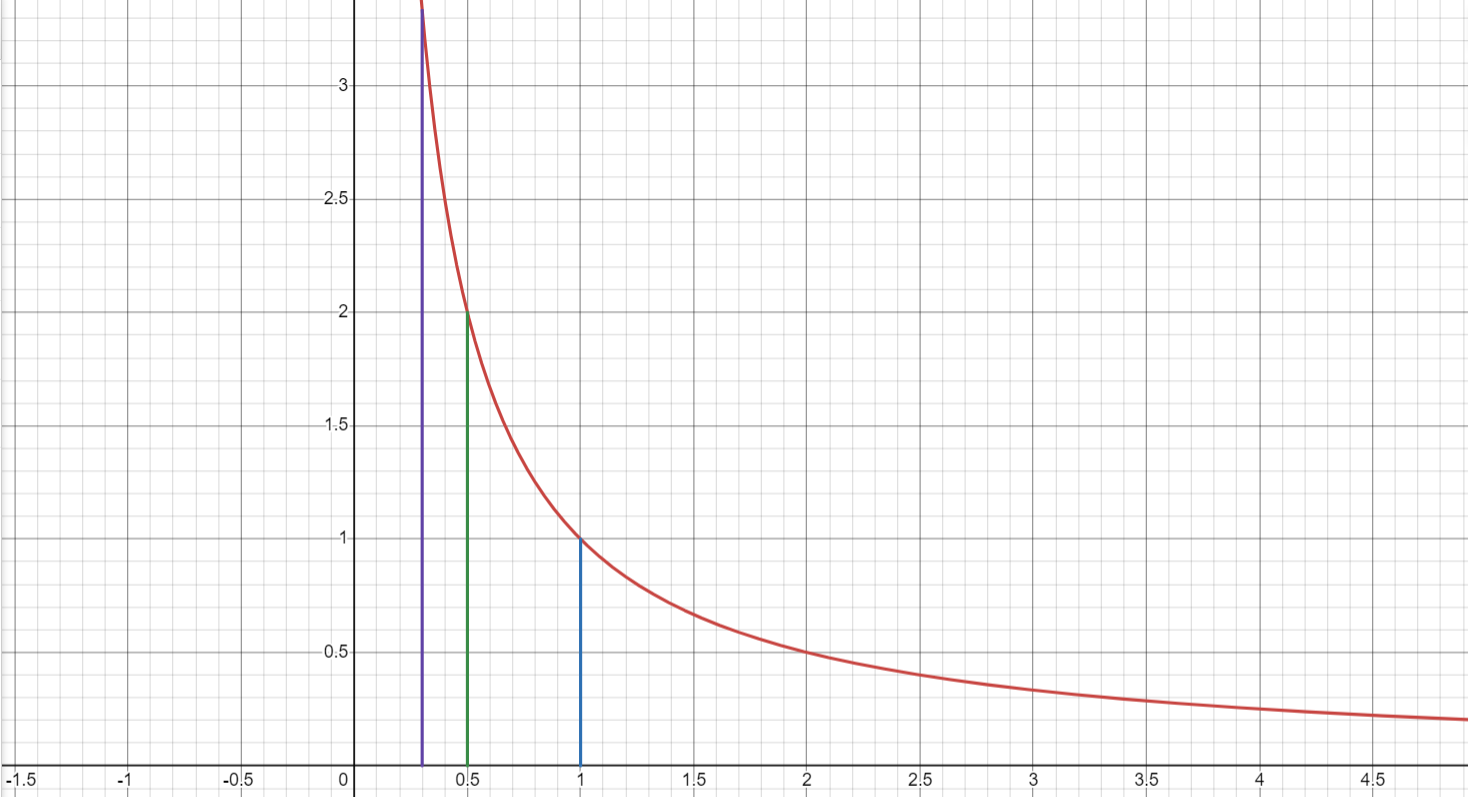
\includegraphics[width = 10cm]{pictures/improperintegral1.png}
    \centering
    \caption{Graph of $\frac{1}{x}$}
\end{figure}
Since we know that $f(x) = \frac{1}{x}$ is not defined at $x=0$, we need to use some clever trick to calculate this integral.

Let's rewrite the lower bound as $a$:
\[
    \int_a^1\frac{1}{x}\mathrm{d}x
\]
where $a>0$.

\newpage
However this integral is not equal to the original integral we want to find, since the lower bound is not equal,
but if we take the limit as $a\to 0$, this integral will approach the integral we want to findm the we can apply the fundamental theorem of calculus and find the result:
\[
    \begin{split}
        \lim_{a\to 0^-} \int_{a}^{1}\frac{1}{x}\mathrm{d}x &= \lim_{a\to 0^-}\ln a - \ln 1 \\
        & = \infty - 0 \\
        & = \infty
    \end{split}
\]
Hence we can see that this integral diverges (the limit goes to infinity).

Let's take a look at where the integral converges:
\[
    \int_0^1\frac{1}{\sqrt{x}}\mathrm{d}x
\]
We can apply the same trick we used:
\[
    \begin{split}
        \lim_{a\to 0^-} \int_{a}^{1}\frac{1}{\sqrt{x}}\mathrm{d}x &= \lim_{a\to 0^-} -2\sqrt{a} + 2\sqrt{1} \\
        & = 0 + 2 \\
        & = 2
    \end{split}
\]
Which means this integral converges (the limit has a finite value)

\subsection{Infinite Integration Bound}
We will use some example to illustrate the idea of integrating on a infinte bound:
\[
    \int_{1}^{\infty} \frac{1}{x}\mathrm{d}x
\]
Let's first replace the upper bound to $b$, and note when $b$ become very large, the integral will get very close to the original integral:
\[
    \begin{split}
        \int_{1}^{\infty} \frac{1}{x}\mathrm{d}x & = \lim_{b\to \infty} \int_{1}^{b} \frac{1}{x}\mathrm{d}x\\
        & = \lim_{b\to \infty} \ln b - \ln 1 \\
        & = \infty - 0\\
        & = \infty
    \end{split}
\]

Which means this integral diverges, we can see that there is no difference between this improper integral and the one listed above, it is both taking a limit, the same also apply for negative infinity,
the lower bound will approach negative infinity.

Let's see a integral that converges:
\[
    \int_{1}^{\infty} \frac{1}{x^2}\mathrm{d}x
\]
\[
    \begin{split}
        \int_{1}^{\infty} \frac{1}{x^2}\mathrm{d}x & = \lim_{b\to \infty} \int_{0}^{b}\frac{1}{x^2}\mathrm{d}x\\
        & = \lim_{b\to \infty} -\frac{1}{b} + 1 \\
        & = 1
    \end{split}
\]

\subsection{Both Infinite Discontinuity and Infinite Integration Bound}
There are other improper integral that can be seen as a combination of both case 1 and case 2,
but first, lets take a look at this theorem
\[
    \text{Let} \int_{a}^{b} f(x)\mathrm{d}x \text{ be an improper integral, } 
    \text{the integral only converges if } \int_{a}^{c} f(x)\mathrm{d}x \text{ and } \int_{c}^{b} f(x)\mathrm{d}x \text{ both converges}
\]
This gives a method to calculate some other improper integrals:
\[
    \int_{-\infty}^{\infty} \frac{1}{1+x^2}\mathrm{d}x
\]
We can rewrite the integral as:
\[
    \begin{split}
        \int_{-\infty}^{\infty} \frac{1}{1+x^2}\mathrm{d}x & = \int_{-\infty}^{0} \frac{1}{1+x^2}\mathrm{d}x + \int_{0}^{\infty} \frac{1}{1+x^2} \mathrm{d}x \\
        & = \lim_{b\to -\infty} \int_{b}^{0} \frac{1}{1+x^2}\mathrm{d}x + \lim_{a\to \infty} \int_{0}^{a}\frac{1}{1+x^2}\mathrm{d}x\\
        & = \arctan 0 - \lim_{b\to -\infty} \arctan b + \arctan 0 - \lim_{a\to \infty} \arctan a \\
        & = -\frac{-\pi}{2} + \frac{\pi}{2} \\
        & = \pi
    \end{split}
\]
Which means this integral converges to $\pi$.

\[
    \int_{0}^{\infty} \frac{1}{x^2}\mathrm{d}x
\]
It is convenient to split this integral into two parts and analyze them separately:
\[
    \begin{split}
        \int_{0}^{\infty} \frac{1}{x^2}\mathrm{d}x &= \int_{0}^{1}\frac{1}{x^2}\mathrm{d}x + \int_{1}^{\infty}\frac{1}{x^2} \mathrm{d}x\\
        & = \lim_{b\to 0^+} \int_{b}^{1} \frac{1}{x^2}\mathrm{d}x + \lim_{a\to \infty} \int_{1}^{a} \frac{1}{x^2} \mathrm{d}x \\
        & = -\frac{1}{1} + \lim_{b\to 0^+} \frac{1}{b} + 1\\
        & = \infty
    \end{split}
\]

There is a quicker way to do this:
\[
    \begin{split}
        \int_{0}^{1}\frac{1}{x^2}\mathrm{d}x & = -\frac{1}{1} + \lim_{b\to 0^+} \frac{1}{b} \\
        & = -1 + \infty \\
        & = \infty \\
    \end{split}
\]
This integral diverges, which by the theorem introduce earlier, the entire integral diverges.

Pretty much all improper integral can be split like this and examine separately to see if they converge or diverge.

\newpage
\section{Determining the convergence of improper integral}
Sometimes it is not convenient to apply the fundamental theorem of calculus to evaluate the improper integral, so we introduce some alernative method to test the convergence of an integral.

Note that all the theorem metioned below \textbf{requires that in the interval $(a,b)$, there is only one infinite discontinuity and it is either $a$ or $b$. Also all the function must be positive in the bound of integration}
\subsection{Direct comparison test}
Let's first understand it graphically:
\begin{figure}[H]
    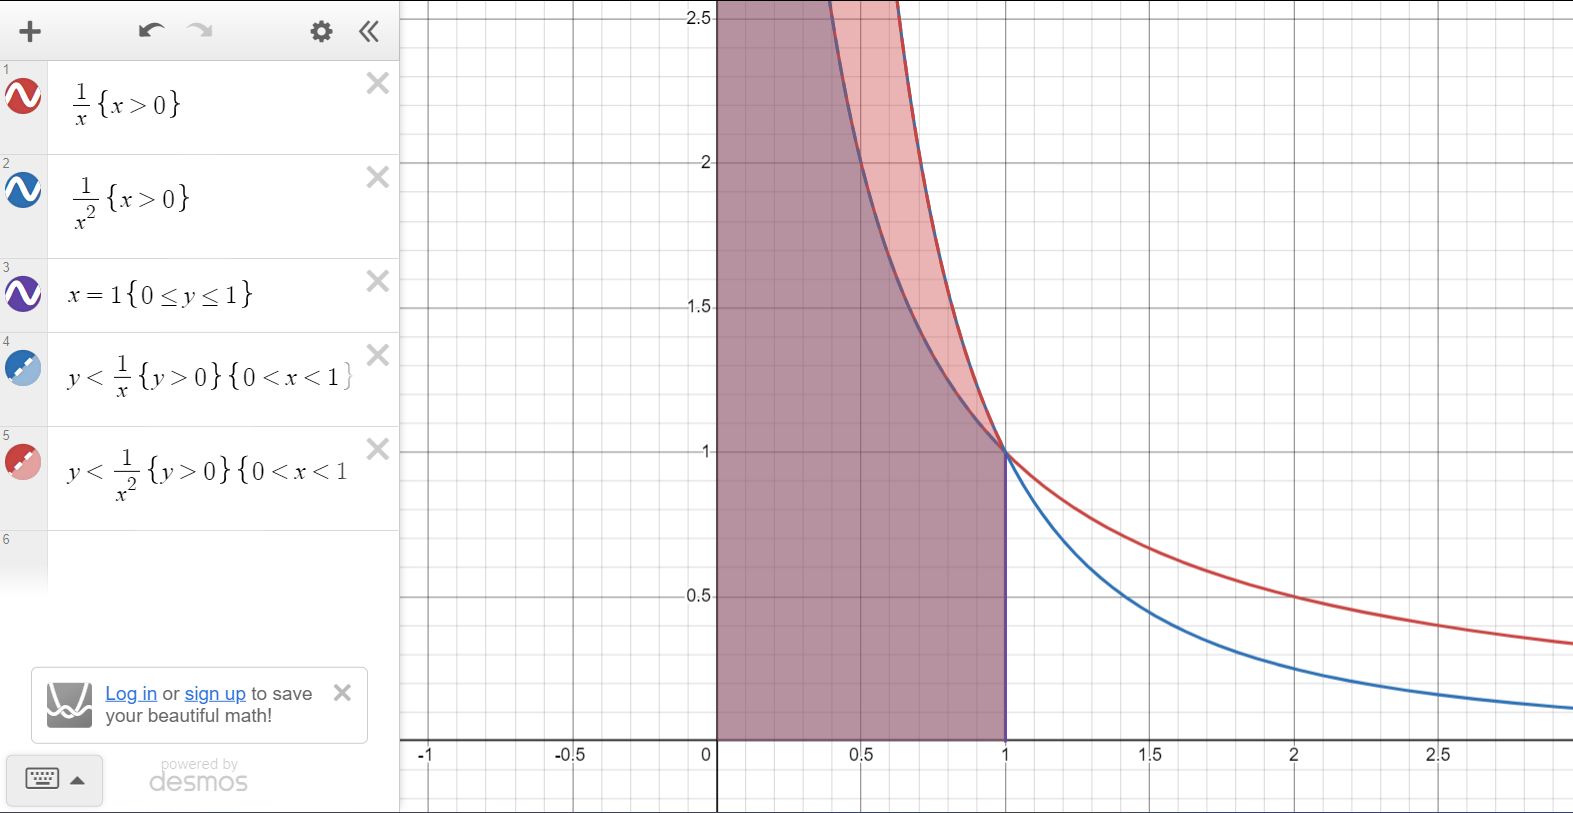
\includegraphics[width = 12cm]{pictures/improperintegral2}
    \centering
\end{figure}
The blue curve is $f(x) = \frac{1}{x^2}$ and the red curve is $g(x) = \frac{1}{x}$. We can see that the area under $f(x)$ is bigger than the area under $g(x)$ from $(0,1)$, or:

\[
    \int_{0}^{1}\frac{1}{x^2}\mathrm{d}x \geq \int_{0}^{1}\frac{1}{x}\mathrm{d}x
\]
Since we know that $\int_{0}^{1}\frac{1}{x}\mathrm{d}x$ is divergent, that means:
\[
    \int_{0}^{1}\frac{1}{x^2}\mathrm{d}x \geq \infty
\]

Which only has one possibility:
\[
    \int_{0}^{1}\frac{1}{x^2}\mathrm{d}x = \infty
\]
This leads to our first theorem, the Direct Comparison Test:
\[
    \text{if } 0 \leq g(x) \leq f(x) \text{ in the interval } [a,b) \text{ and } \int_{a}^{b} f(x) \mathrm{d}x \text{ converges, then} \int_{a}^{b} g(x) \mathrm{d}x \text{ also converges}
\]
\[
    \text{if } 0 \leq g(x) \leq f(x) \text{ in the interval } [a,b) \text{ and } \int_{a}^{b} g(x) \mathrm{d}x \text{ diverges, then} \int_{a}^{b} f(x) \mathrm{d}x \text{ also diverges}
\]

\newpage
\subsection{Limit comparison test}
Let's see the theorem first:
\[
    \text{For } \lim_{x\to a} \frac{f(x)}{g(x)} = C \text{ is a positive integer and } a \text{ is a infinite discontinuity}
\]
\[
    \text{Then } \int_{a}^{b} f(x)\mathrm{d}x \text{and} \int_{a}^{b} g(x)\mathrm{d}x \text{ converge or diverge at the same time}
\]
A good example to start will be:
\[
    \int_{0}^{1} \frac{1}{\sin \sqrt{x}}\mathrm{d}x
\]
It is very difficult to find the integral of this function, and it is impossible to use the direct comparison test, but we do know that:
\[
    \lim_{x\to 0}\frac{\sin \sqrt{x}}{\sqrt{x}} = 1
\]
Which means we can replace $\sin \sqrt{x}$ with $\sqrt{x}$ and get this integral:
\[
    \int_{0}^{1}\frac{1}{\sqrt{x}}\mathrm{d}x
\]
Which is proven to be convergent, meaning our original integral is also converges.

Another example would be
\[
    \int_{0}^{1}\csc x \ \mathrm{d}x = \int_{0}^{1} \frac{1}{\sin x} \mathrm{d}x
\]

It is obvious that:
\[
    \lim_{x\to 0}\frac{\sin x}{x} = 1
\]
Which means we can replace $\sin x$ with $\frac{1}{x}$ and get this integral:
\[
    \int_{0}^{1}\frac{1}{x} \ \mathrm{d}x
\]
This integral diverges, so our original integral also diverges.

\newpage
\subsection{P-Series Test}
There are 2 situation for p-series test:

\begin{enumerate}
    \item For any finite $a>0$, the integral:
    \[
        \int_{a}^{\infty} \frac{1}{x^p} \mathrm{d}x
    \]
    converges if $p>1$, diverges if $p\leq 1$
    \item For any finite $a>0$, the integral:
    \[
        \int_{0}^{a} \frac{1}{x^p} \mathrm{d}x
    \]
    converges if $p<1$, diverges if $p\geq 1$.
\end{enumerate}
Sometimes it is difficult to Rememeber this theorem because there are 2 cases and for each case, the converge criteria is different. Here is the trick:

Remember that
\[
    \int_{a}^{\infty}\frac{1}{x^2}\mathrm{d}x \text{ converges, } 
    \int_{0}^{a}\frac{1}{\sqrt{x}}\mathrm{d}x \text{ also converges. }
\]

Then by p-series test, we have:
\[
    \int_{0}^{a}\frac{1}{x^2}\mathrm{d}x \text{ diverges, } 
    \int_{a}^{\infty}\frac{1}{\sqrt{x}}\mathrm{d}x \text{ also diverges. }
\]

An interesting example will be:
\[
    \int_{1}^{\infty} \frac{1}{x^{1.0000000001}}\mathrm{d}x
\]
Since $1.0000000001>1$, this integral converges, despite how close $1.0000000001$ and $1$ is.

Note, if you really can't remember, just derive it, its not that deep.

\newpage
\subsection{Absolute Convergence Method}
Theorem:
\[
    \text{If } \int_{a}^{b} |f(x)| \mathrm{d}x \text{ converges, then } \int_{a}^{b} f(x) \mathrm{d}x \text{ converges.}
\]
This theorem is extremely useful when the function is not always positive in the integration bound, a good example would be:
\[
    \int_{1}^{\infty}\frac{\sin x}{x^2}\mathrm{d}x
\]
This integral is not always positive since $-1\leq \sin x \leq 1$ and $x^2\geq 0$, it is convenient for us to use absolute convergence method, consider this integral:
\[
    \int_{1}^{\infty} \abs{\frac{\sin x}{x^2}} \mathrm{d}x = \int_{1}^{\infty} \frac{\abs{\sin x}}{x^2} \mathrm{d}x
\]
We know that 
\[  
    \frac{\abs{\sin x}}{x^2} \leq \frac{1}{x^2}
\]
Then by direct comparison test, we have:
\[
    \int_{1}^{\infty} \frac{\abs{\sin x}}{x^2} \mathrm{d}x \leq \int_{1}^{\infty} \frac{1}{x^2} \mathrm{d}x
\]
We know $\int_{1}^{\infty} \frac{1}{x^2} \mathrm{d}x$ converges, so $ \int_{1}^{\infty} \frac{\abs{\sin x}}{x^2} \mathrm{d}x$ also converge. By the theorem we introduced:
\[
    \int_{1}^{\infty}\frac{\sin x}{x^2}\mathrm{d}x \text{ also converge}
\]

Note that this method can only prove that the \textbf{integral converges, it cannot prove that the integral diverges}, for example:
\[
    \text{If } \int_{a}^{b} |f(x)| \mathrm{d}x \text{ diverges, } \int_{a}^{b} f(x) \mathrm{d}x \text{ don't necessarily diverges.}
\]

\newpage
\section{Examples of Different Types of Improper Integral}
\subsection{Polynomials}
Consider this integral:
\[
    \int_{1}^{\infty} \frac{1}{2+20\sqrt{x}}\mathrm{d}x
\]
First, there is only one infinity discontinuity, which is at $\infty$, so we don't have to split this integral into more parts.

Notice that 
\[
    \lim_{x\to \infty} \frac{2+20\sqrt{x}}{20\sqrt{x}} = 1
\]
Which means we can replace the integrand by limit comparison test:
\[
    \int_{1}^{\infty} \frac{1}{20\sqrt{x}} \mathrm{d}x
\]
By p-series test, this integral diverges, so 
\[
    \int_{1}^{\infty} \frac{1}{2+20\sqrt{x}}\mathrm{d}x \text{ diverges}
\]

A pattern we can find is if $ax^n$ is the highest order term in the polynomial $p(x)$, then:
\[
    \lim_{x\to \infty} \frac{p(x)}{ax^n} = 1
\]
This identity also holds true for $x\to -\infty$, this relation is very handy since we now can use limit comparison test for polynomial improper integral.

Another integral we will look at is:
\[
    \int_{0}^{\infty} \frac{1}{x^5+4x^4+1}\mathrm{d}x
\]
We can see that $x^{5}$ is the highest order term in the polynomial of $x^5+4x^4+1$, which means we can replace the integral like this:
\[
    \int_{0}^{\infty} \frac{1}{x^5}\mathrm{d}x
\]
However, the new integrand of $1/x^5$ have a infinity discontinuity at $x=0$, which our original integrand does not have, so before replacing the integrand, we need to split it up:
\[
\begin{split}
    \int_{0}^{\infty} \frac{1}{x^5+4x^4+1}\mathrm{d}x & = \int_{0}^{1} \frac{1}{x^5+4x^4+1}\mathrm{d}x + \int_{1}^{\infty} \frac{1}{x^5+4x^4+1}\mathrm{d}x\\
    & = \int_{0}^{1} \frac{1}{x^5+4x^4+1}\mathrm{d}x + \int_{1}^{\infty} \frac{1}{x^5} \mathrm{d}x
\end{split}
\]
The first integral is not even an improper integral, so it must converge, by p-series test, the second integral converges, meaning 
\[
    \int_{0}^{\infty} \frac{1}{x^5+4x^4+1}\mathrm{d}x \text{ converges}
\]

\newpage
\subsection{Trig functions}
Two very important relations holds true from $\sin$ and $\cos$:
\[
    \abs{\sin A}\leq 1 \text{ and } \abs{\cos A} \leq 1
\]
The first use of these inequalities is using direct comparison test to find the convergence of integrals:
\[
    \int_{5}^{\infty} \frac{\abs{\sin x^4}}{x^2 + \sqrt{x}} \mathrm{d} x
\]
By the inequality listed, we have 
\[
    \int_{5}^{\infty} \frac{\abs{\sin x^4}}{x^2 + \sqrt{x}} \mathrm{d} x \leq \int_{5}^{\infty} \frac{1}{x^2 + \sqrt{x}} \mathrm{d} x
\]
We can replace $x^2+\sqrt{x}$ to $x^2$ to simplify our calculations (\textbf{note the replaced integral does not equal to the original integral}) and get
\[
    \int_{5}^{\infty} \frac{1}{x^2} \mathrm{d}x
\]
This integral converge, and using direct comparison method
\[
    \int_{5}^{\infty} \frac{\abs{\sin x^4}}{x^2 + \sqrt{x}} \mathrm{d} x \text{ converge}
\]

Another interesting use of the inequalities is we can ignore $\sin x^n$ or $cos x^n$ even if $n$ is really big
\[
    \int_{8}^{\infty} \frac{1}{2x^3 -3x^{0.1} + \sin {100x^{200}}} \mathrm{d}x
\]
Since $\abs{\sin A}\leq 1$, $2x^3 -3x^{0.1} + \sin {100x^{200}}$ can be replaced by $2x^3$ and the integral become
\[
    \int_{8}^{\infty} \frac{1}{2x^3}\mathrm{d}x
\]
This integral converges, which means that 
\[
    \int_{8}^{\infty} \frac{1}{2x^3 -3x^{0.1} + \sin {100x^{200}}} \mathrm{d}x \text{ converges}
\] 
\end{document}